\chapter{Hàm sóng của dao động tử, spin một phần hai và sự trao đổi hạt}

\section{Dao động tử ở khắp nơi}

Mọi hệ có trạng thái cân bằng bền đều có thể dao động khi bị dịch chuyển khỏi trạng thái cân bằng đó. Hệ có thể có một hoặc nhiều tần số. Chẳng hạn, dây đàn violin có mode cơ bản và các họa âm bậc cao. Khi gảy dây, ta kích thích một tổ hợp các mode ấy.

Những ví dụ quan trọng hơn ở đây là các trường. Cấu hình cân bằng của trường điện từ là chân không: không có điện trường, không có từ trường và không có dao động điện từ. Đưa bức xạ vào một hốc cộng hưởng hoặc ống dẫn sóng thì trường có thể dao động ở các mode được phép, mỗi mode có tần số riêng. Trong lý thuyết lượng tử, các mode ấy mô tả những tập hợp photon.

Ý tưởng tương tự cũng áp dụng cho tinh thể. Hình dung mỗi nguyên tử là một dao động tử độc lập sẽ gây hiểu lầm. Các nguyên tử tác dụng lực lên nhau, nên khi một nguyên tử dịch chuyển, các nguyên tử lân cận cũng bị ảnh hưởng và một sóng lan truyền qua tinh thể. Các mode chuẩn của chuyển động liên kết đó là những dao động tử điều hòa, còn lượng tử của chúng được gọi là phonon. Photon và phonon là những đối tượng vật lý khác nhau, nhưng cả hai đều dẫn trở lại cùng một đại số dao động tử.

\section{Đại số dao động tử}

Trong phần bàn về dao động tử, lấy khối lượng và hằng số Planck rút gọn bằng một:
\[
m=1,\qquad \hbar=1.
\]
Hamiltonian là
\begin{equation}
H=\frac{p^{2}}{2}+\frac{\omega^{2}x^{2}}{2}.
\end{equation}
Tham số \(\omega\) xác định độ cong của thế năng, đồng thời cũng là tần số dao động.

Định nghĩa các toán tử nâng và hạ như sau:
\begin{equation}
A_{\pm}=\frac{p\pm i\omega x}{\sqrt{2\omega}}.
\end{equation}
Chọn chuẩn hóa sao cho
\begin{equation}
[A_{-},A_{+}]=1.
\end{equation}
Toán tử số là
\begin{equation}
N=A_{+}A_{-}.
\end{equation}
Các phương trình này cùng suy ra rằng \(A_{+}\) làm tăng một đơn vị trị riêng của \(N\), còn \(A_{-}\) làm giảm trị riêng đó một đơn vị. Phổ thu được là
\begin{equation}
n=0,1,2,3,\ldots .
\end{equation}

Nhân hai toán tử bậc thang với nhau cũng cho thấy hiệu chỉnh lượng tử đối với năng lượng cổ điển:
\begin{align}
N
&=\frac{1}{2\omega}(p+i\omega x)(p-i\omega x)\\
&=\frac{1}{2\omega}\left(p^{2}+\omega^{2}x^{2}
 +i\omega[x,p]\right)\\
&=\frac{1}{2\omega}\left(p^{2}+\omega^{2}x^{2}-\omega\right),
\end{align}
trong đó \([x,p]=i\). Do đó,
\begin{equation}
H=\omega\left(N+\frac12\right).
\end{equation}
Nếu hằng số cộng không liên quan đến bài toán, ta có thể dùng Hamiltonian đã dịch:
\begin{equation}
H_{\mathrm{shifted}}=H-\frac{\omega}{2}=\omega N.
\end{equation}
Số hạng \(\omega/2\) là năng lượng điểm không, hay năng lượng trạng thái cơ bản, của dao động tử. Với một mode trường, số hạng tương tự được gọi là năng lượng chân không. Nó phản ánh nguyên lý bất định: không trạng thái nào có thể đồng thời có \(x\) và \(p\) bằng không một cách xác định, nên cả hai số hạng bậc hai dương trong \(H\) không thể cùng có giá trị kỳ vọng bằng không.

\begin{classroomqa}
\lecturetimestamp{00:09:46}
\audiencequestion{Vì sao số không được tính vào phổ của toán tử số?}
\lecturerresponse{Có thể chứng minh điều này một cách tường minh bằng cách dựng hàm sóng trạng thái cơ bản. Phép dựng đó sẽ cho thấy có một trạng thái thỏa \(N=0\).}
\end{classroomqa}

Để bắt đầu phép dựng ấy, thay các vectơ trạng thái bằng các hàm sóng theo vị trí. Các trạng thái riêng năng lượng trở thành
\[
\psi_{0}(x),\ \psi_{1}(x),\ \psi_{2}(x),\ldots,
\]
và các toán tử cơ bản tác dụng như sau:
\begin{equation}
X\longmapsto x,\qquad
P\longmapsto -i\frac{d}{dx}.
\end{equation}
Khi khôi phục \(\hbar\), phép thay thứ hai sẽ là
\(P\mapsto-i\hbar\,d/dx\).

Trước khi giải tìm \(\psi_{0}\), ta có thể trả lời câu hỏi bằng lập luận trừu tượng nhanh hơn. Trên thang rời rạc gồm các trạng thái riêng chuẩn hóa được của dao động tử, \(N=A_{+}A_{-}\) không âm, nên không thể tiếp tục hạ liên tiếp từng đơn vị mãi mãi. Ở điểm cuối---mà hàm sóng chuẩn hóa được sẽ được dựng bên dưới---, phải có một trạng thái, ký hiệu là \(\lvert0\rangle\), sao cho
\begin{equation}
A_{-}\lvert0\rangle=\mathbf 0.
\end{equation}
Nếu không thì \(A_{-}\lvert0\rangle\) sẽ là một trạng thái khác thấp hơn một bậc. Suy ra ngay rằng
\begin{equation}
N\lvert0\rangle
=A_{+}A_{-}\lvert0\rangle
=\mathbf 0
=0\,\lvert0\rangle.
\end{equation}
Vậy trạng thái thấp nhất có trị riêng số bằng không.

\begin{classroomqa}
\lecturetimestamp{00:14:57}
\audiencequestion{Nếu trị riêng bằng không, vế phải có nên chứa một vectơ riêng không?}
\lecturerresponse{Ket \(\lvert0\rangle\) là một vectơ chuẩn hóa khác không có nhãn bằng không. Trong \(N\lvert0\rangle=0\,\lvert0\rangle\), vế phải là vectơ không. Ket trạng thái cơ bản và vectơ không là hai đối tượng khác nhau.}
\end{classroomqa}

\section{Phương trình Schr\"odinger và các nghiệm vật lý}

Giờ hãy trở lại biểu diễn theo vị trí. Phương trình Schr\"odinger không phụ thuộc thời gian là
\begin{equation}
\left[
-\frac12\frac{d^{2}}{dx^{2}}
+\frac12\omega^{2}x^{2}
\right]\psi(x)=E\psi(x).
\end{equation}
Là một phương trình vi phân bậc hai, nó có các nghiệm hình thức ứng với mọi giá trị \(E\). Phần lớn các nghiệm hình thức ấy không phải là trạng thái vật lý của dao động tử. Chúng tăng theo hàm mũ khi \(\lvert x\rvert\) lớn, khiến chuẩn của chúng phân kỳ.

Với một trạng thái liên kết, hàm sóng phải bình phương khả tích:
\begin{equation}
\int_{-\infty}^{\infty}\psi^{*}(x)\psi(x)\,dx<\infty.
\end{equation}
Sau đó có thể chuẩn hóa hàm sóng để tích phân bằng một. Chỉ những giá trị năng lượng đặc biệt mới cho các nghiệm như vậy. Các trạng thái vị trí và động lượng trên đường thẳng vô hạn là những trường hợp ngoại lệ về mặt này, còn các nghiệm dao động tử tăng theo hàm mũ thì đơn giản là bị loại khỏi không gian trạng thái.

\section{Trạng thái cơ bản dạng Gaussian}

Có thể giải phương trình bậc hai, nhưng đại số bậc thang cho một phương trình bậc nhất đơn giản hơn:
\begin{equation}
A_{-}\psi_{0}(x)=0.
\end{equation}
Khi vế phải bằng không, hệ số tổng thể trong \(A_{-}\) không ảnh hưởng, nên phương trình này tương đương với
\begin{equation}
(p-i\omega x)\psi_{0}(x)=0.
\end{equation}
Dùng \(p=-i\,d/dx\), ta được
\begin{equation}
\left(\frac{d}{dx}+\omega x\right)\psi_{0}(x)=0.
\end{equation}

\begin{classroomqa}
\lecturetimestamp{00:22:32}
\audiencequestion{Có thể giải phương trình này bằng phương pháp phân ly biến số không?}
\lecturerresponse{Ở đây chỉ có một biến độc lập, nên không có hai biến để phân ly. Viết dưới dạng \(\psi_{0}'/\psi_{0}=-\omega x\), phương trình có dạng của một đạo hàm logarithm. Điều đó gợi ý biểu diễn hàm sóng dưới dạng hàm mũ.}
\end{classroomqa}

Một cách giải hữu ích là đặt
\begin{equation}
\psi_{0}(x)=e^{f(x)}.
\end{equation}
Khi đó,
\[
\psi_{0}'(x)=f'(x)e^{f(x)},
\]
và thừa số hàm mũ chung triệt tiêu. Phương trình rút gọn thành
\begin{equation}
\frac{df}{dx}+\omega x=0.
\end{equation}

\begin{classroomqa}
\lecturetimestamp{00:26:28}
\audiencequestion{Trong \(f(x)\) có nên có dấu trừ không?}
\lecturerresponse{Có. Vì \(df/dx=-\omega x\), phép tích phân cho một số hạng bậc hai mang dấu âm.}
\end{classroomqa}

Do đó,
\begin{equation}
f(x)=-\frac12\omega x^{2}+C,
\end{equation}
và
\begin{equation}
\psi_{0}(x)\propto e^{-\omega x^{2}/2}.
\end{equation}
Ta chưa xác định hằng số nhân chuẩn hóa. Điều quan trọng là dạng Gaussian: hàm này trơn, tập trung gần gốc tọa độ và giảm nhanh khi \(\lvert x\rvert\) lớn. Rõ ràng nó bình phương khả tích.

Không cần thế đáp án trở lại phương trình bậc hai để tìm năng lượng. Đại số đã cho ta
\begin{equation}
E_{0}=\frac{\omega}{2}.
\end{equation}

\section{Trạng thái kích thích, nút và chuyển động cổ điển}

Trạng thái kích thích thứ nhất thu được bằng cách nâng trạng thái cơ bản:
\begin{equation}
\psi_{1}(x)\propto A_{+}\psi_{0}(x)
\propto(p+i\omega x)e^{-\omega x^{2}/2}.
\end{equation}
Phương trình trạng thái cơ bản cho biết
\[
p\psi_{0}=i\omega x\,\psi_{0}.
\]
Đổi dấu trong toán tử bậc thang biến sự triệt tiêu thành phép cộng:
\begin{equation}
(p+i\omega x)\psi_{0}
=2i\omega x\,\psi_{0}.
\end{equation}
Bỏ qua một hằng số tổng thể,
\begin{equation}
\psi_{1}(x)\propto x\,e^{-\omega x^{2}/2}.
\end{equation}

Hàm sóng này là hàm lẻ:
\begin{equation}
\psi_{1}(-x)=-\psi_{1}(x).
\end{equation}
Mật độ xác suất của nó là hàm chẵn, nhưng có một nút tại gốc tọa độ:
\begin{equation}
\lvert\psi_{1}(0)\rvert^{2}=0.
\end{equation}
Vậy mật độ xác suất của trạng thái kích thích thứ nhất có một nút tại \(x=0\).

Tác dụng lặp lại của \(A_{+}\) cho các đa thức bậc cao hơn nhân với cùng một bao Gaussian.\footnote{Bài giảng nêu các thừa số đa thức bậc cao, nút bổ sung ở mỗi bước và tính chẵn lẻ luân phiên từ \(00{:}34{:}25\) đến \(00{:}35{:}49\). Dạng tích của Gaussian với đa thức được Leonard Susskind và Art Friedman xác nhận trong \emph{Cơ học lượng tử: Những kiến thức tối thiểu} (2014), ở phần bàn về các hàm riêng của dao động tử.} Bỏ qua chuẩn hóa,
\begin{equation}
\psi_{n}(x)=P_{n}(x)e^{-\omega x^{2}/2}.
\end{equation}
Tính chẵn lẻ luân phiên giữa chẵn và lẻ, và mỗi bước làm tăng thêm một nút. Khi \(n\) tăng, hàm sóng trải rộng ra xa gốc hơn và dao động nhanh hơn.

Hai đặc điểm này có ý nghĩa vật lý trực tiếp. Hàm sóng có biên độ đáng kể ở xa gốc hơn tương ứng với thế năng lớn hơn, vì thế năng tăng theo \(x^{2}\). Dao động nhanh trong không gian vị trí báo hiệu động lượng lớn hơn. Một dao động tử kích thích mạnh có khả năng vươn xa tâm hơn; khi đi qua vùng trung tâm, nó mang động lượng lớn hơn và hàm sóng dao động nhanh hơn ở vùng đó.

\begin{classroomqa}
\lecturetimestamp{00:37:18}
\audiencequestion{Khi \(n\) lớn, dao động tử điều hòa có tiến gần đến hành vi cổ điển không?}
\lecturerresponse{Chuyển động cổ điển không được biểu diễn bởi một trạng thái riêng năng lượng dừng duy nhất. Nó xuất hiện trong một gói sóng gồm nhiều mức năng lượng. Chẳng hạn, một Gaussian bị dịch chuyển tiến hóa qua lại như một dao động tử cổ điển, và độ bất định tương đối giảm khi biên độ dao động tăng.}
\end{classroomqa}

Bắt đầu với Gaussian của trạng thái cơ bản rồi dịch chuyển nó khỏi gốc. Gói sóng sau khi dịch chuyển không còn là trạng thái riêng năng lượng nữa; nó là chồng chập của nhiều trạng thái như vậy. Theo phương trình Schr\"odinger phụ thuộc thời gian, các thành phần của gói sóng thu được những pha khác nhau. Gói sóng dao động từ bên này sang bên kia của thế năng, phát triển biến thiên pha nhanh gần tâm và trở nên trơn trở lại gần điểm quay. Biên độ dao động càng lớn so với độ rộng của gói sóng thì chuyển động biểu hiện càng gần với chuyển động cổ điển.

\begin{classroomqa}
\lecturetimestamp{00:39:29}
\audiencequestion{Hàm sóng của trạng thái kích thích thứ hai có đi qua không tại gốc tọa độ không?}
\lecturerresponse{Không. Thừa số đa thức của nó không chỉ gồm \(x^{2}\); nó còn chứa một số hạng hằng, nên hàm sóng không nhất thiết triệt tiêu tại \(x=0\).}
\end{classroomqa}

Lập luận bậc thang cũng giả định rằng \(A_{+}\) và \(A_{-}\) là các toán tử liên hợp Hermite trên miền dao động tử gồm các hàm bình phương khả tích, với điều kiện biên cần thiết để quan hệ liên hợp đúng. Các nghiệm hình thức tăng theo hàm mũ không thuộc miền đó.

\begin{classroomqa}
\lecturetimestamp{00:40:45}
\audiencequestion{Có cách tổng quát nào để nhận biết một Hamiltonian có thể giải được bằng các phương pháp đại số hay không?}
\lecturerresponse{Không có quy tắc tổng quát như vậy. Các ví dụ giải được chính xác rất hiếm. Dao động tử điều hòa và nguyên tử hydro phi tương đối tính lý tưởng là những trường hợp may mắn mà các phương pháp đại số có hiệu quả.}
\end{classroomqa}

\section{Spin một phần hai như động lượng góc}

Spin là động lượng góc do hạt mang, độc lập với chuyển động quỹ đạo của khối tâm. Hạt đứng yên không có động lượng góc quỹ đạo \(\mathbf R\times\mathbf P\), nhưng vẫn có thể có spin. Có thể thử hình dung hạt như một vật nhỏ đang quay, hoặc xem spin là một tính chất lượng tử nội tại. Phát biểu quyết định mang tính toán học: các thành phần spin biến đổi dưới phép quay không gian và tuân theo các hệ thức giao hoán của động lượng góc.

Từ đây trở đi, khôi phục \(\hbar\). Các thành phần động lượng góc thỏa mãn
\begin{equation}
[L_{z},L_{x}]=i\hbar L_{y},
\end{equation}
Hai hệ thức còn lại thu được bằng cách hoán vị vòng. Các ma trận Pauli không thứ nguyên là
\begin{equation}
\begin{aligned}
\sigma_{z}&=
\begin{pmatrix}
1&0\\
0&-1
\end{pmatrix},\\[0.4em]
\sigma_{x}&=
\begin{pmatrix}
0&1\\
1&0
\end{pmatrix},\\[0.4em]
\sigma_{y}&=
\begin{pmatrix}
0&-i\\
i&0
\end{pmatrix}.
\end{aligned}
\end{equation}
Trong cơ sở này, \(\sigma_{z}\) là ma trận đường chéo. Các trị riêng của nó là \(+1\) và
\(-1\).

\begin{classroomqa}
\lecturetimestamp{00:47:35}
\audiencequestion{Trong \(\sigma_x\) có dấu trừ không?}
\lecturerresponse{Không. Hai phần tử ngoài đường chéo của \(\sigma_x\) đều dương.}
\end{classroomqa}

Phép tính trên bảng tại \(00{:}49{:}35\) bắt đầu quá trình nhân từng phần tử.
Thực hiện đầy đủ các phép nhân, ta được
\begin{align}
\sigma_{z}\sigma_{x}
&=
\begin{pmatrix}
0&1\\
-1&0
\end{pmatrix}
=i\sigma_{y},\\
\sigma_{x}\sigma_{z}
&=
\begin{pmatrix}
0&-1\\
1&0
\end{pmatrix}
=-i\sigma_{y}.
\end{align}
Do đó,
\begin{equation}
[\sigma_{z},\sigma_{x}]=2i\sigma_{y}.
\end{equation}
Thừa số hai dư ra được loại bỏ bằng cách định nghĩa các toán tử spin vật lý như sau:\footnote{Phép tính trên bảng bỏ qua \(\hbar\). Ở đây khôi phục đại lượng này để \(S_i\) có đơn vị động lượng góc.}
\begin{equation}
S_{i}=\frac{\hbar}{2}\sigma_{i}.
\end{equation}
Khi đó,
\begin{equation}
[S_{z},S_{x}]=i\hbar S_{y},
\end{equation}
và tương tự với các phép hoán vị vòng. Vì vậy, một nửa các ma trận Pauli, sau khi khôi phục thừa số \(\hbar\), tạo thành một hệ động lượng góc.

Đặt \(\hbar=1\) thì thu được dạng trình bày dưới đây.\footnote{Khung nguồn là \texttt{bài giảng\_04\_khung\_02.png}.}
\begin{figure}[htbp]
\centering
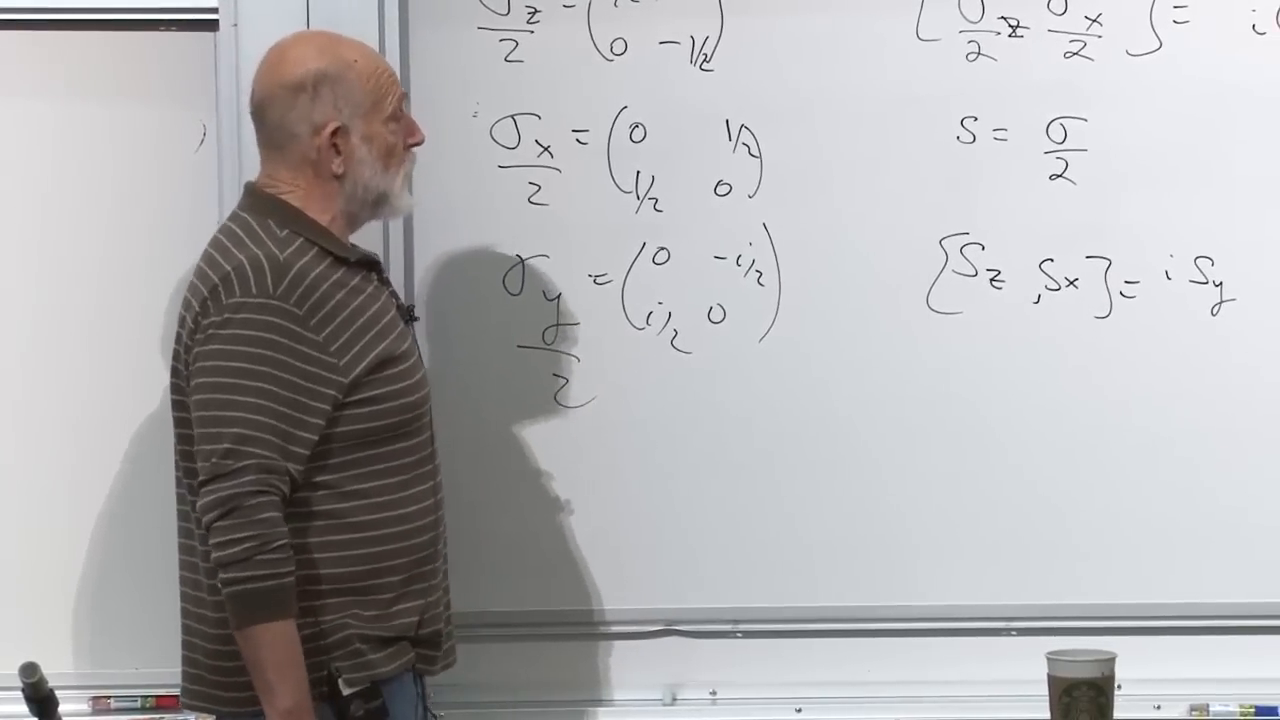
\includegraphics[width=0.9\linewidth]{lecture_04_frame_02.png}
\caption{Trong đơn vị \(\hbar=1\), một nửa các ma trận Pauli là các toán tử động lượng góc spin một phần hai và thỏa mãn \([S_z,S_x]=iS_y\).}
\lectureframe{00:55:41}
\end{figure}

Hai phương trình trị riêng \(S_z\) là
\begin{equation}
S_z\lvert\pm\rangle
=\pm\frac{\hbar}{2}\lvert\pm\rangle.
\end{equation}
Tương đương, số lượng tử từ không thứ nguyên là
\begin{equation}
m_{s}=\pm\frac12,
\qquad
S_{z}\lvert m_{s}\rangle
=m_{s}\hbar\,\lvert m_{s}\rangle.
\end{equation}
Các toán tử nâng và hạ của động lượng góc dịch chuyển \(m\) theo các bước nguyên, nhưng điều đó không có nghĩa là mọi thang đều phải đi qua số không. Các đa tuyến nguyên chứa các giá trị \(m\) nguyên, còn các đa tuyến bán nguyên chứa các giá trị bán nguyên. Với spin một phần hai, thang chỉ có hai thành viên \(m_s=+1/2\) và \(m_s=-1/2\).

Hai trạng thái này tạo thành bộ đôi spin một phần hai. Electron, muon, neutrino và quark là những hạt thuộc các đa tuyến spin bán nguyên như vậy.

\section{Động lượng góc quỹ đạo và spin}

Giờ đây ta có hai loại động lượng góc. Động lượng góc quỹ đạo mô tả chuyển động tương đối so với một gốc tọa độ,
\begin{equation}
\mathbf L=\mathbf R\times\mathbf P,
\end{equation}
trong khi \(\mathbf S\) là spin nội tại. Tổng vectơ của chúng là động lượng góc toàn phần:
\begin{equation}
\mathbf J=\mathbf L+\mathbf S.
\end{equation}

\begin{classroomqa}
\lecturetimestamp{00:56:49}
\audiencequestion{Nếu một hệ có động lượng góc toàn phần \(\mathbf J\), làm thế nào xác định spin \(\mathbf S\) của hệ?}
\lecturerresponse{Thông thường, số lượng tử spin và số lượng tử quỹ đạo được cho riêng. Nếu \(L=0\), toàn bộ động lượng góc là spin. Nếu không, cần dùng các quy tắc lượng tử để cộng động lượng góc; phần này sẽ bàn đến sau.}
\end{classroomqa}

Các quy tắc cộng áp dụng như nhau cho tổng của động lượng góc quỹ đạo với spin, cho hai spin hoặc cho hai động lượng góc quỹ đạo. Hệ tổ hợp có các giá trị động lượng góc toàn phần được phép riêng, nhưng hiện chưa cần đến các quy tắc đó.

\begin{classroomqa}
\lecturetimestamp{00:58:18}
\audiencequestion{Bằng chứng thực nghiệm nào đã dẫn đến việc đưa spin vào lý thuyết?}
\lecturerresponse{Quang phổ học đã cung cấp bằng chứng, nhưng bảng tuần hoàn đem lại một lý do đặc biệt rõ ràng: cấu trúc lớp electron đòi hỏi electron phải có thêm một tính chất hai giá trị.}
\end{classroomqa}

\section{Suy biến kiểu hydro và phép đếm lớp}

Với động lượng góc quỹ đạo, phương trình trị riêng \(L^{2}\) là
\begin{equation}
L^{2}\lvert\ell,m\rangle
=\hbar^{2}\ell(\ell+1)\lvert\ell,m\rangle,
\end{equation}
và một giá trị cố định của \(\ell\) có
\begin{equation}
2\ell+1
\end{equation}
trạng thái từ, tương ứng với \(m=-\ell,-\ell+1,\ldots,\ell\).

Bài toán Coulomb phi tương đối tính lý tưởng có thêm một suy biến. Các mức năng lượng liên kết âm và tiến đến không từ phía dưới, nhưng khi đếm, chỉ cần xét sự trùng mức. Mức \(\ell=1\) thứ nhất trùng với mức \(\ell=0\) kế tiếp; mức \(\ell=2\) thứ nhất nhập vào lớp chính kế tiếp; và quy luật này tiếp diễn.\footnote{\texttt{bài giảng\_04\_khung\_03.png}, \(01{:}02{:}01\); sự trùng mức hoàn chỉnh giữa các lớp chính được trình bày từ \(01{:}02{:}33\) đến \(01{:}04{:}10\).}

\begin{figure}[htbp]
\centering
\begin{tikzpicture}[x=1.55cm,y=1.0cm]
\draw[->] (-0.65,0) -- (-0.65,4.35);
\draw[->] (-0.85,0) -- (4.75,0);
\node at (-0.95,4.08) {\(E\)};
\node at (4.55,-0.28) {\(\ell\)};
\node at (0,-0.30) {\(0\)};
\node at (2,-0.30) {\(1\)};
\node at (4,-0.30) {\(2\)};

\draw (-0.20,0.75) -- (0.20,0.75);

\draw (-0.20,2.00) -- (0.20,2.00);
\foreach \dx in {-0.18,0,0.18}
  \draw (2+\dx-0.06,2.00) -- (2+\dx+0.06,2.00);

\draw (-0.20,3.15) -- (0.20,3.15);
\foreach \dx in {-0.18,0,0.18}
  \draw (2+\dx-0.06,3.15) -- (2+\dx+0.06,3.15);
\foreach \dx in {-0.32,-0.16,0,0.16,0.32}
  \draw (4+\dx-0.05,3.15) -- (4+\dx+0.05,3.15);

\node[anchor=west] at (0.35,0.75) {\(n=1\)};
\node[anchor=west] at (2.35,2.00) {\(n=2\)};
\node[anchor=west] at (4.40,3.15) {\(n=3\)};
\end{tikzpicture}
\caption{Ba lớp Coulomb lý tưởng đầu tiên gồm các đa tuyến quỹ đạo có cùng năng lượng chính: một trạng thái ở lớp thứ nhất, \(1+3\) ở lớp thứ hai và \(1+3+5\) ở lớp thứ ba.}
\lectureframe{01:02:01}
\end{figure}

Trong lớp chính \(n\), các giá trị động lượng góc quỹ đạo được phép là\footnote{Khoảng \(\ell\) gọn này và tổng bên dưới tái dựng sự trùng mức cùng các số đếm \(1,4,9,16,\ldots\) được trình bày từ \(01{:}02{:}33\) đến \(01{:}04{:}10\). Phần đầu của hình phổ xuất hiện trong \texttt{bài giảng\_04\_khung\_03.png} tại \(01{:}02{:}01\).}
\[
\ell=0,1,\ldots,n-1.
\]
Vì vậy, số trạng thái không gian là
\begin{equation}
\sum_{\ell=0}^{n-1}(2\ell+1)=n^{2},
\end{equation}
cho dãy
\begin{equation}
1,\ 4,\ 9,\ 16,\ldots .
\end{equation}
Đây chỉ là phép đếm các trạng thái quỹ đạo. Mỗi trạng thái không gian cho phép hai giá trị spin, nên các tổng tương ứng trong mô hình lý tưởng hóa là
\begin{equation}
2,\ 8,\ 18,\ 32,\ldots=2n^{2}.
\end{equation}

\section{Nguyên lý loại trừ và tính chất hai giá trị của electron}

Xét helium trong gần đúng electron độc lập. Hạt nhân của nó có điện tích proton gấp đôi, làm thay đổi tỉ lệ các mức kiểu hydro và kéo electron vào gần hơn. Tạm bỏ qua tương tác electron--electron, hai electron có thể chiếm orbital không gian thấp nhất và cho một gần đúng ban đầu hợp lý đối với trạng thái cơ bản của helium.

Vì sao không đặt thêm electron thứ ba vào đó? Làm vậy sẽ hạ năng lượng quỹ đạo của nó, nhưng điều này không xảy ra. Hạn chế ấy là nguyên lý loại trừ Pauli: không hai electron nào được chiếm cùng một trạng thái một hạt đầy đủ. Gọi đây là một lực đẩy thông thường sẽ gây hiểu lầm. Đó là một hạn chế đối với các trạng thái lượng tử được phép.

Thoạt nhìn có vẻ mâu thuẫn. Hai electron trong helium quả thật cùng chiếm một orbital không gian. Lời giải là một trạng thái electron đầy đủ chứa nhiều hơn hàm sóng quỹ đạo. Nó còn chứa một bậc tự do có hai giá trị. Gọi hai giá trị ấy là spin lên và spin xuống. Một electron trong orbital thấp nhất có thể ở trạng thái spin lên, electron kia ở trạng thái spin xuống; trạng thái không gian của chúng giống nhau, nhưng trạng thái lượng tử đầy đủ thì khác nhau.

Đến đây, phép đếm bắt đầu tiến lên phía trước đến lithium rồi quay lại. Việc quay lại làm rõ vì sao cần cả nguyên lý loại trừ lẫn spin. Hãy hình dung một quy tắc loại trừ không có spin. Khi đó chỉ một electron có thể chiếm trạng thái không gian thấp nhất. Electron thứ hai phải đi vào một trong bốn trạng thái không gian thuộc lớp chính kế tiếp, tạo ra vài khả năng khác nhau trong khi trạng thái cơ bản helium quan sát được là duy nhất. Phiên bản nguyên lý loại trừ không có spin ấy là sai.

Khôi phục hai giá trị spin. Hai electron lấp đầy orbital thấp nhất với spin ngược chiều nhau. Electron thứ ba, như trong lithium trung hòa, phải đi vào lớp chính kế tiếp. Lớp đó có một trạng thái không gian \(\ell=0\) và ba trạng thái không gian \(\ell=1\). Trước khi tính đến spin, có bốn khả năng.

\begin{classroomqa}
\lecturetimestamp{01:14:58}
\audiencequestion{Các trạng thái \(s\) và \(p\) tạo ra tám khả năng trong lớp kích thích đầu tiên như thế nào?}
\lecturerresponse{Có một trạng thái không gian với \(\ell=0\) và ba trạng thái với \(\ell=1\), tức là có bốn trạng thái không gian. Mỗi trạng thái cho phép hai giá trị spin, nên tổng số là \(2(1+3)=8\).}
\end{classroomqa}

Đây là phép đếm đơn giản giải thích tám vị trí ở hàng thứ hai của bảng tuần hoàn. Đây chủ ý là một mô hình lý tưởng hóa: phần bàn luận sau sẽ làm rõ rằng tương tác electron--electron sớm phá vỡ hình ảnh các lớp hydro độc lập.

Cũng có thể kiểm tra tính chất hai giá trị này dưới góc độ động lượng góc. Spin của electron đi kèm với mômen từ, nên từ trường làm cho hai hình chiếu spin có năng lượng khác nhau. Một mức vốn suy biến khi không có từ trường sẽ tách thành hai mức, đúng như dự đoán đối với một mômen từ nhỏ định hướng song song hoặc ngược chiều với từ trường. Sự tách mức kiểm tra xem bậc tự do hai giá trị được thêm vào có hành xử như động lượng góc hay chỉ là một nhãn nhị phân tùy ý.

\section{Photon, electron và giới hạn của mô hình lớp}

Không phải mọi hạt đều tuân theo cùng một quy tắc chiếm chỗ. Nhiều photon có thể chiếm cùng một mode điện từ; có thể hiểu sóng ánh sáng cổ điển là một trạng thái chứa số lượng lớn photon trong mode đó. Electron thì khác: nguyên lý loại trừ ngăn chúng cùng dồn vào một trạng thái lượng tử đầy đủ. Sự tương phản này dẫn đến phân biệt giữa hai loại thống kê hạt.

\begin{classroomqa}
\lecturetimestamp{01:20:28}
\audiencequestion{Nếu xét một chùm electron tự do thay vì các electron liên kết trong nguyên tử thì sao?}
\lecturerresponse{Quy tắc loại trừ vẫn áp dụng: các electron không thể cùng chiếm một trạng thái lượng tử. Laser có thể đưa nhiều photon vào cùng một mode, nhưng không thể chuẩn bị chùm electron theo cách ấy.}
\end{classroomqa}

Hạn chế này là tính chất của electron, không phải đặc điểm riêng của sự liên kết trong nguyên tử.

\begin{classroomqa}
\lecturetimestamp{01:21:12}
\audiencequestion{Động lượng góc quỹ đạo có nhất thiết là chuyển động quay quanh hạt nhân không?}
\lecturerresponse{Động lượng góc được xác định tương đối với một gốc tọa độ đã chọn. Trong nguyên tử, hạt nhân là gốc tự nhiên, còn hạt tự do có động lượng góc \(\mathbf R\times\mathbf P\) tương đối với gốc tọa độ tùy ý được chọn.}
\end{classroomqa}

Mọi bàn luận về phép quay đều chọn một điểm làm tâm quay. Nguyên tử có một tâm tự nhiên, vì hạt nhân là tâm của thế gần như thế trung tâm. Trong không gian tự do, không có gốc tọa độ nào được ưu tiên, dù ta vẫn có thể tính động lượng góc quanh bất kỳ gốc nào được chọn.

\begin{classroomqa}
\lecturetimestamp{01:22:34}
\audiencequestion{Vì sao bảng tuần hoàn có những hàng lặp lại gồm tám nguyên tố rồi đến những hàng lặp lại gồm mười tám nguyên tố?}
\lecturerresponse{Mô hình lớp electron độc lập đơn giản không giải thích được toàn bộ quy luật. Mô hình nhanh chóng không còn phù hợp vì bỏ qua tương tác giữa các electron.}
\end{classroomqa}

Trong một nguyên tử lớn, các electron ngoài tương tác với đám mây electron bên trong đáng kể cũng như với hạt nhân. Không còn hợp lý nếu xem mỗi electron như thể nó chuyển động độc lập trong trường Coulomb không bị che chắn.

\begin{classroomqa}
\lecturetimestamp{01:23:33}
\audiencequestion{Vì sao kích thước nguyên tử không tăng lên đáng kể khi thêm nhiều electron?}
\lecturerresponse{Thêm electron cũng đồng nghĩa với thêm proton vào hạt nhân. Điện tích hạt nhân tăng lên kéo các electron bên trong về gần hơn, trong khi các electron bên trong che chắn hạt nhân. Theo mô hình đơn giản này, một electron hóa trị ở ngoài sẽ chuyển động trong điện tích hiệu dụng xấp xỉ bằng một.}
\end{classroomqa}

Điện tích hạt nhân tăng lên làm đám mây bên trong co lại. Với nguyên tử có một electron hóa trị ở ngoài, ở khoảng cách lớn, điện tích hạt nhân và các electron bên trong gần như triệt tiêu nhau, khiến electron hóa trị ở trong trường gần giống trường của một điện tích dương đơn vị. Vì vậy, kích thước nguyên tử không đơn giản tăng tỉ lệ với số electron.

\begin{classroomqa}
\lecturetimestamp{01:24:49}
\audiencequestion{Lực đẩy điện có phải là lý do khiến các nguyên tử lân cận cách xa nhau không?}
\lecturerresponse{Không phải chỉ do lực này. Nguyên lý loại trừ Pauli tạo ra một lực đẩy hiệu dụng quan trọng khi các đám mây electron chồng lấn; với nhiều nguyên tử, đây là lý do chủ yếu khiến chúng chống lại sự chồng lấn thêm.}
\end{classroomqa}

Lực đẩy Pauli là hệ quả hiệu dụng của nguyên lý loại trừ, không phải một định luật lực bổ sung.

\begin{classroomqa}
\lecturetimestamp{01:25:23}
\audiencequestion{Nguyên lý loại trừ có phải là một tiên đề riêng không?}
\lecturerresponse{Trong cơ học lượng tử phi tương đối tính, nguyên lý này được đặt làm tiên đề. Trong lý thuyết lượng tử tương đối tính, mối liên hệ spin--thống kê tạo cho nguyên lý một nền tảng sâu xa hơn.}
\end{classroomqa}

\section{Hạt đồng nhất trong cơ học cổ điển và cơ học lượng tử}

Trước khi phát biểu tiên đề đó, hãy xét cách đếm hạt đồng nhất trong cơ học cổ điển. Đặt hai hạt cùng loại vào một tập hợp các hộp. Nếu các hạt bí mật mang tên riêng---Harry và Sally---thì Harry ở hộp thứ nhất và Sally ở hộp thứ hai dường như là một cấu hình khác với Sally ở hộp thứ nhất và Harry ở hộp thứ hai.

Cơ học cổ điển cho phép hình dung như vậy ngay cả khi các nhãn mờ đến mức không thể phát hiện. Ta có thể tưởng tượng trên mỗi hạt có một dấu hiệu yếu tùy ý mà vẫn xem quỹ đạo của chúng là khác nhau. Trong cơ học thống kê cổ điển, người ta thường chọn không tính các hoán vị của những hạt đồng nhất thành cấu hình mới. Với \(N\) hạt, quy ước này cho thừa số quen thuộc \(1/N!\).

Cơ học lượng tử nghiêm ngặt hơn. Về nguyên tắc, hạt đồng nhất không mang nhãn cá thể ẩn để ta có thể theo dõi. Hai electron có thể hoán đổi cho nhau với tư cách electron. Hoán đổi một electron với một photon sẽ tạo ra cấu hình vật lý khác vì chúng là hai loại hạt khác nhau, nhưng hoán đổi hai vị trí electron không thể cho biết electron nào thực ra là electron nào.

Một trạng thái một hạt có hàm sóng
\[
\psi(x)=\langle x\vert\psi\rangle.
\]
Với hai hạt, trạng thái là một hàm của hai đối số vị trí:
\begin{equation}
\psi(x_{1},x_{2}).
\end{equation}
Các chỉ số dưới đánh dấu hai vị trí trong mô tả, không phải hai phương hướng không gian. Bình phương môđun của hàm cho mật độ xác suất vị trí đồng thời.

\section{Toán tử hoán đổi và tiên đề thống kê}

Hoán đổi hai vị trí hạt:
\begin{equation}
\psi(x_{1},x_{2})\longmapsto\psi(x_{2},x_{1}).
\end{equation}
Theo ký hiệu dùng trong phần này, gọi toán tử hoán đổi là \(S\). Ở đây \(S\) ký hiệu phép hoán đổi, không phải vectơ spin \(\mathbf S\). Toán tử tác dụng như sau:
\begin{equation}
(S\psi)(x_{1},x_{2})=\psi(x_{2},x_{1}).
\end{equation}
Một hàm tổng quát của hai biến không nhất thiết đối xứng, nên phép toán này có thể tạo ra một hàm sóng khác.

Hoán đổi hai lần thì khôi phục thứ tự ban đầu:
\begin{equation}
S^{2}=I.
\end{equation}
Phép hoán đổi thuận nghịch và bảo toàn tích vô hướng, nên được biểu diễn bởi một toán tử unita. Nếu \(\psi\) là một vectơ riêng của \(S\) với trị riêng \(\lambda\), thì
\[
S^{2}\psi=\lambda^{2}\psi=\psi,
\]
và do đó
\begin{equation}
\lambda=\pm1.
\end{equation}

Kết luận này xác định hai không gian riêng của phép hoán đổi, nhưng không khẳng định rằng mọi hàm sóng hai hạt bất kỳ đều đã là vectơ riêng của \(S\). Có thể phân tách mọi hàm sóng như vậy thành hai phần,\footnote{Phép phân tích này là sự làm rõ đại số mang tính biên tập về hai không gian riêng được hàm ý bởi \(S^{2}=I\). Lập luận được ghi lại nêu hai trị riêng rồi đưa ra nguyên lý thống kê bổ sung.}\begin{equation}
\psi_{\pm}=\frac12(I\pm S)\psi,
\end{equation}
thỏa mãn
\begin{equation}
S\psi_{\pm}=\pm\psi_{\pm}.
\end{equation}
Do đó
\begin{align}
\psi_{+}(x_{2},x_{1})&=\psi_{+}(x_{1},x_{2}),\\
\psi_{-}(x_{2},x_{1})&=-\psi_{-}(x_{1},x_{2}).
\end{align}

Tiếp theo là một nguyên lý bổ sung, chứ không phải hệ quả chỉ từ \(S^{2}=I\). Đối với các hạt đồng nhất thuộc cùng một loài xác định, các trạng thái được phép hoàn toàn nằm trong một trong hai phân không gian hoán đổi này: hoán đổi một cặp hạt luôn cho lại cùng một hàm sóng, hoặc luôn cho lại hàm sóng đối của nó. Phân không gian \(+1\) là đối xứng, còn phân không gian \(-1\) là phản đối xứng. Bước tiếp theo là diễn giải vật lý hai khả năng này thành hai loại thống kê hạt; phần thảo luận sau sẽ trình bày điều đó.
